
\section{Tessellation}

敷き詰めはテセレーション(Tessellation),タイリング(Tiling)とも呼ばれる.例えば図は黒の基本領域を周囲の円盤の反転で移した敷き詰め模様と考えることもできる.タイリングは幾何学の重要の道具であると同時に,装飾やアートとしても非常に人気のある分野である.
この章では,シェーダを用いてタイリングを描く方法とその他の参考文献について少しであるがまとめる.

\subsection{About Rendering}

図のような正方形のタイリングを考える.
図のように,基本となる正方形を縦横全4種類の変換の組み合わせで平面全体を正方形で埋め尽くすことができる.これは前章で紹介した,変換の木構造の幅優先探索で正方形を移動して描画することができる.
GLSLを用いる場合はその逆を行う.すなわち,各ピクセルを敷き詰めを構成する4種の変換で基本タイルへと点を動かす.
そうして,基本タイルへ動かした後で操作の回数や基本タイル状の色を参照し描画する.
このアルゴリズムをまとめると以下のような手順になる
\begin{enumerate}
 \item 基本タイルを見つける
 \item 基本タイルを敷き詰めるための変換を見つける
 \item 各ピクセルを基本タイルに入るまで変換し続ける
 \item 変換の回数や基本タイル上の色を使って色を付ける
\end{enumerate}

\begin{figure}[h!tbp]
   \begin{subfigure}{0.3\textwidth}
   \begin{center}
    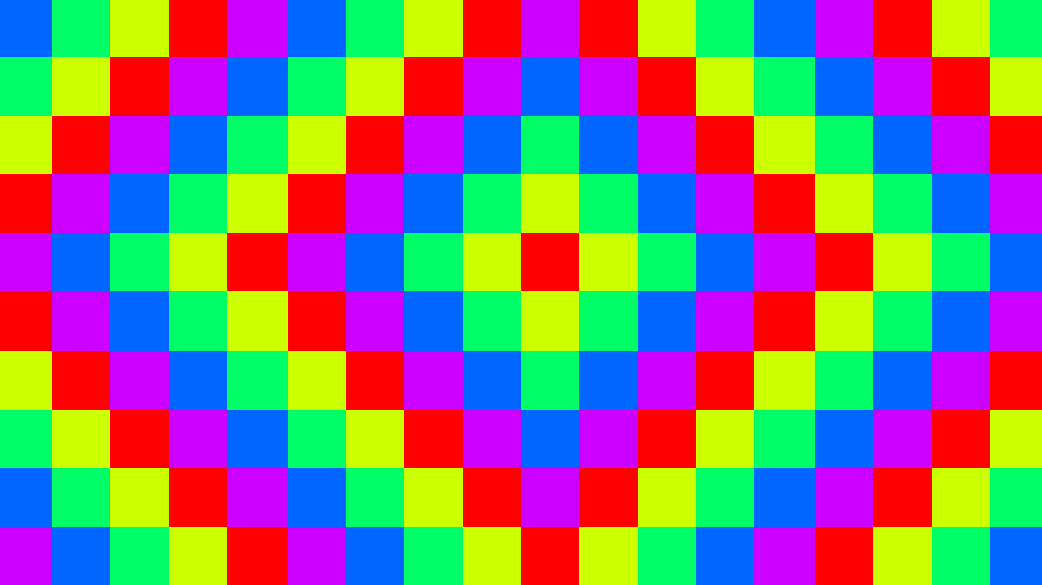
\includegraphics[width=2in, height=2in, keepaspectratio]{../img/tessellation/rectTile.pdf}
    \caption{rectangular tiling}
    \label{fig:rectTile}
   \end{center}
  \end{subfigure}
 \hspace*{\fill}
   \begin{subfigure}{0.3\textwidth}
   \begin{center}
    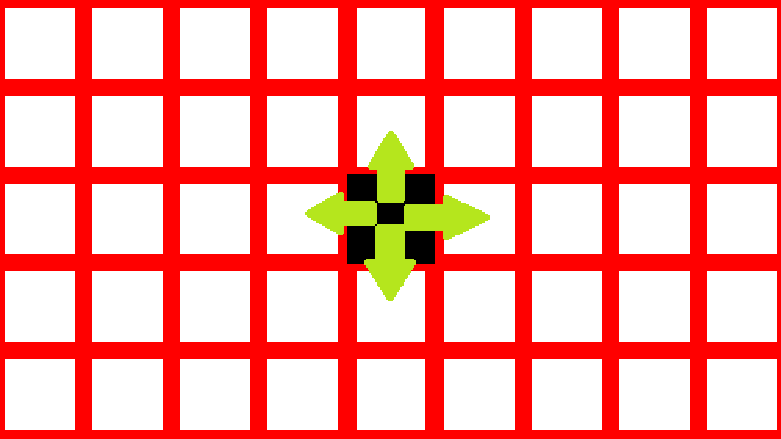
\includegraphics[width=2in, height=2in, keepaspectratio]{../img/tessellation/tile.pdf}
    \caption{Tiling}
    \label{fig:tile}
   \end{center}
  \end{subfigure}
 \hspace*{\fill}
 \begin{subfigure}{0.3\textwidth}
  \begin{center}
   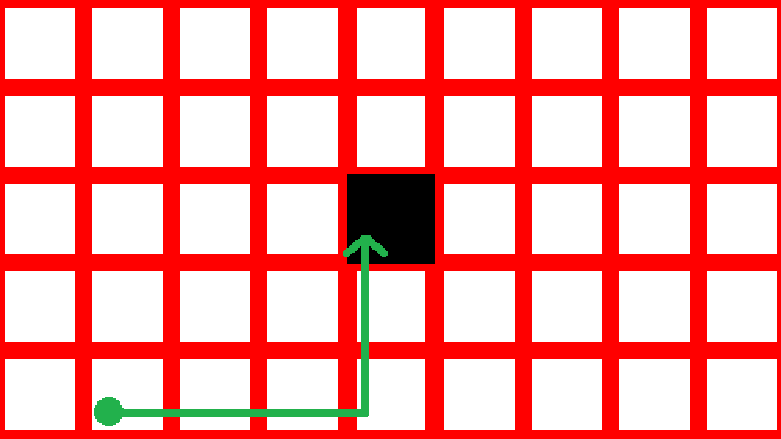
\includegraphics[width=2in, height=2in, keepaspectratio]{../img/tessellation/tileMove.pdf}
   \caption{Move}
   \label{fig:tileMove}
  \end{center}
 \end{subfigure}
 \hspace*{\fill}
\caption{Tile}
\end{figure}

ユークリッド平面状での敷き詰め模様は,数学的に分類がされている.『装飾パターンの法則』\cite{tessellationDesign}では装飾に用いられる敷き詰め模様の法則を解説するとともにデザインへの応用についてもまとめられている.
\cite{hyperbolization}はユークリッド平面上での敷き詰めを双曲平面での敷き詰めに変換する方法についてまとめられている.また,著者が書いたmorenaments\footnote{morenaments: \url{http://www.morenaments.de/}}は各敷き詰めパターンの挙動をみることができる.

\subsection{Hyperbolic Tessellation}
双曲タイリングは双曲平面上での
双曲幾何学では,ポアンカレの円盤モデルと呼ばれる.円盤の端がユークリッド平面における無限遠点となり,円弧がこの平面における直線だと考えられる.また,三角形の和が180度以下になるなどの興味深い現象もみられる.
この平面における敷き詰めが双曲タイリング(Hyperbolic Tessellation)と呼ばれ,画家のエッシャーはこの図に影響されて有名な『天使と悪魔』や『Circle Limit』といった作品を生み出した.

図\ref{fig:poincare}の半球の内側にある円盤がポアンカレの円盤モデルの円盤である.直線を半径が無限の円盤の円周だとみなすと,あらゆるタイルが円弧で構成されていることがわかる.
円盤の内側と外側は円に関する反転で移りあう.
幾何学的には内側も外側も同じものとして扱う.

円盤は原点中心,半径1の円とする.中央の最も大きなタイルはx軸,y軸,そして2つの円弧で囲まれた領域である.
これらの弧に関する反転を用いて,先ほどのアルゴリズムを用いると図\ref{fig:outer}のような敷き詰め模様を描くことができる.
円盤の内側に属する点は内側の基本タイルに,円盤の外側に属する点は外側の基本タイルに移るため,最終的な点の位置で処理を切り分けることにより,両者の色を区別することができる.
双曲タイリングは,木構造の探索によって計算しようとすると,計算量が多くなるため,円盤の端まで描画することは難しいが,前述のアルゴリズムを用いると端までリアルタイムで描画することができる.

図\ref{fig:outer}では基本タイルとして,3つの角が$\frac{\pi}{2}$,残りの角が$\frac{\pi}{3}$である4辺形を用いたが,基本タイルでも敷き詰めることができるわけではない.
敷き詰め条件はポアンカレの張り合わせ定理として知られている.双曲三角形のタイリング条件は以下のようになる.
\begin{eqnarray*}
\text{3内角を}\frac{\pi}{p},\frac{\pi}{q},\frac{\pi}{r}\text{とする時,}
 \frac{1}{p} + \frac{1}{q} + \frac{1}{r} < 1 \text{を満たす.}
\end{eqnarray*}
双曲三角形を2つ張り合わせることで双曲4辺形を得ることができる.

Vladimir Bulatov氏は円盤を変形させる方法を考案した\cite{bending}.Bulatov氏は双曲平面や双曲空間におけるタイリングや,その変形についてまとめている\footnote{Bulatov Abstract Creations: \url{http://bulatov.org/math/index.html}}.
筆者は図\ref{fig:deformed}のような双曲タイリングとその変形を行うWebアプリケーションを制作している.
\footnote{Hyperbolic Tessellator: \url{https://soma-arc.net/HyperbolicTessellator/}}.


\begin{figure}[h!tbp]
 \begin{minipage}{0.49\hsize}
   \begin{center}
    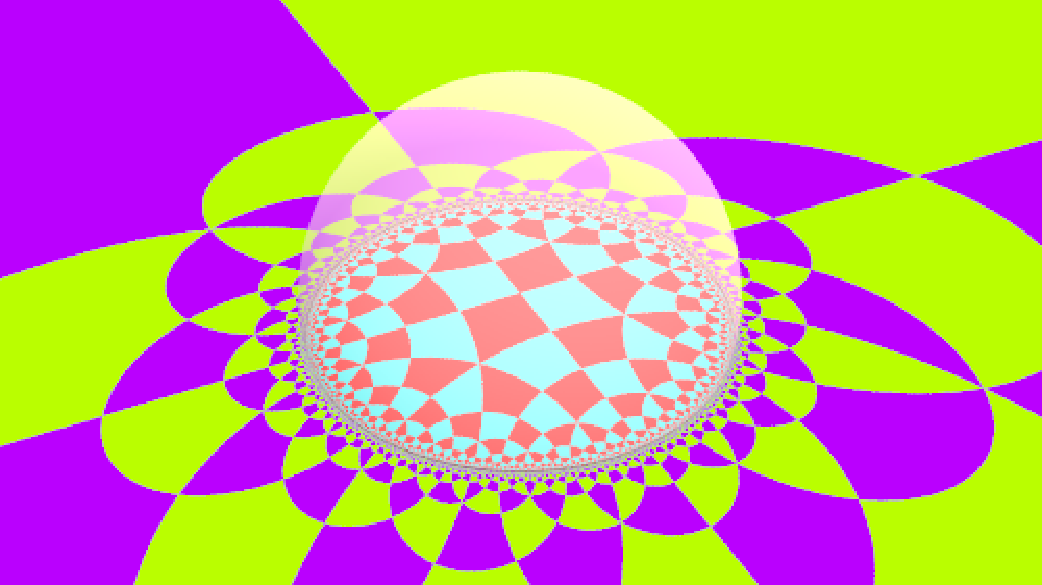
\includegraphics[width=3in, height=3in, keepaspectratio]{../img/tessellation/poincare.pdf}
    \caption{Poincare disk}
    \label{fig:poincare}
   \end{center}
 \end{minipage}
 \hspace*{\fill}
 \begin{minipage}{0.49\hsize}
   \begin{center}
    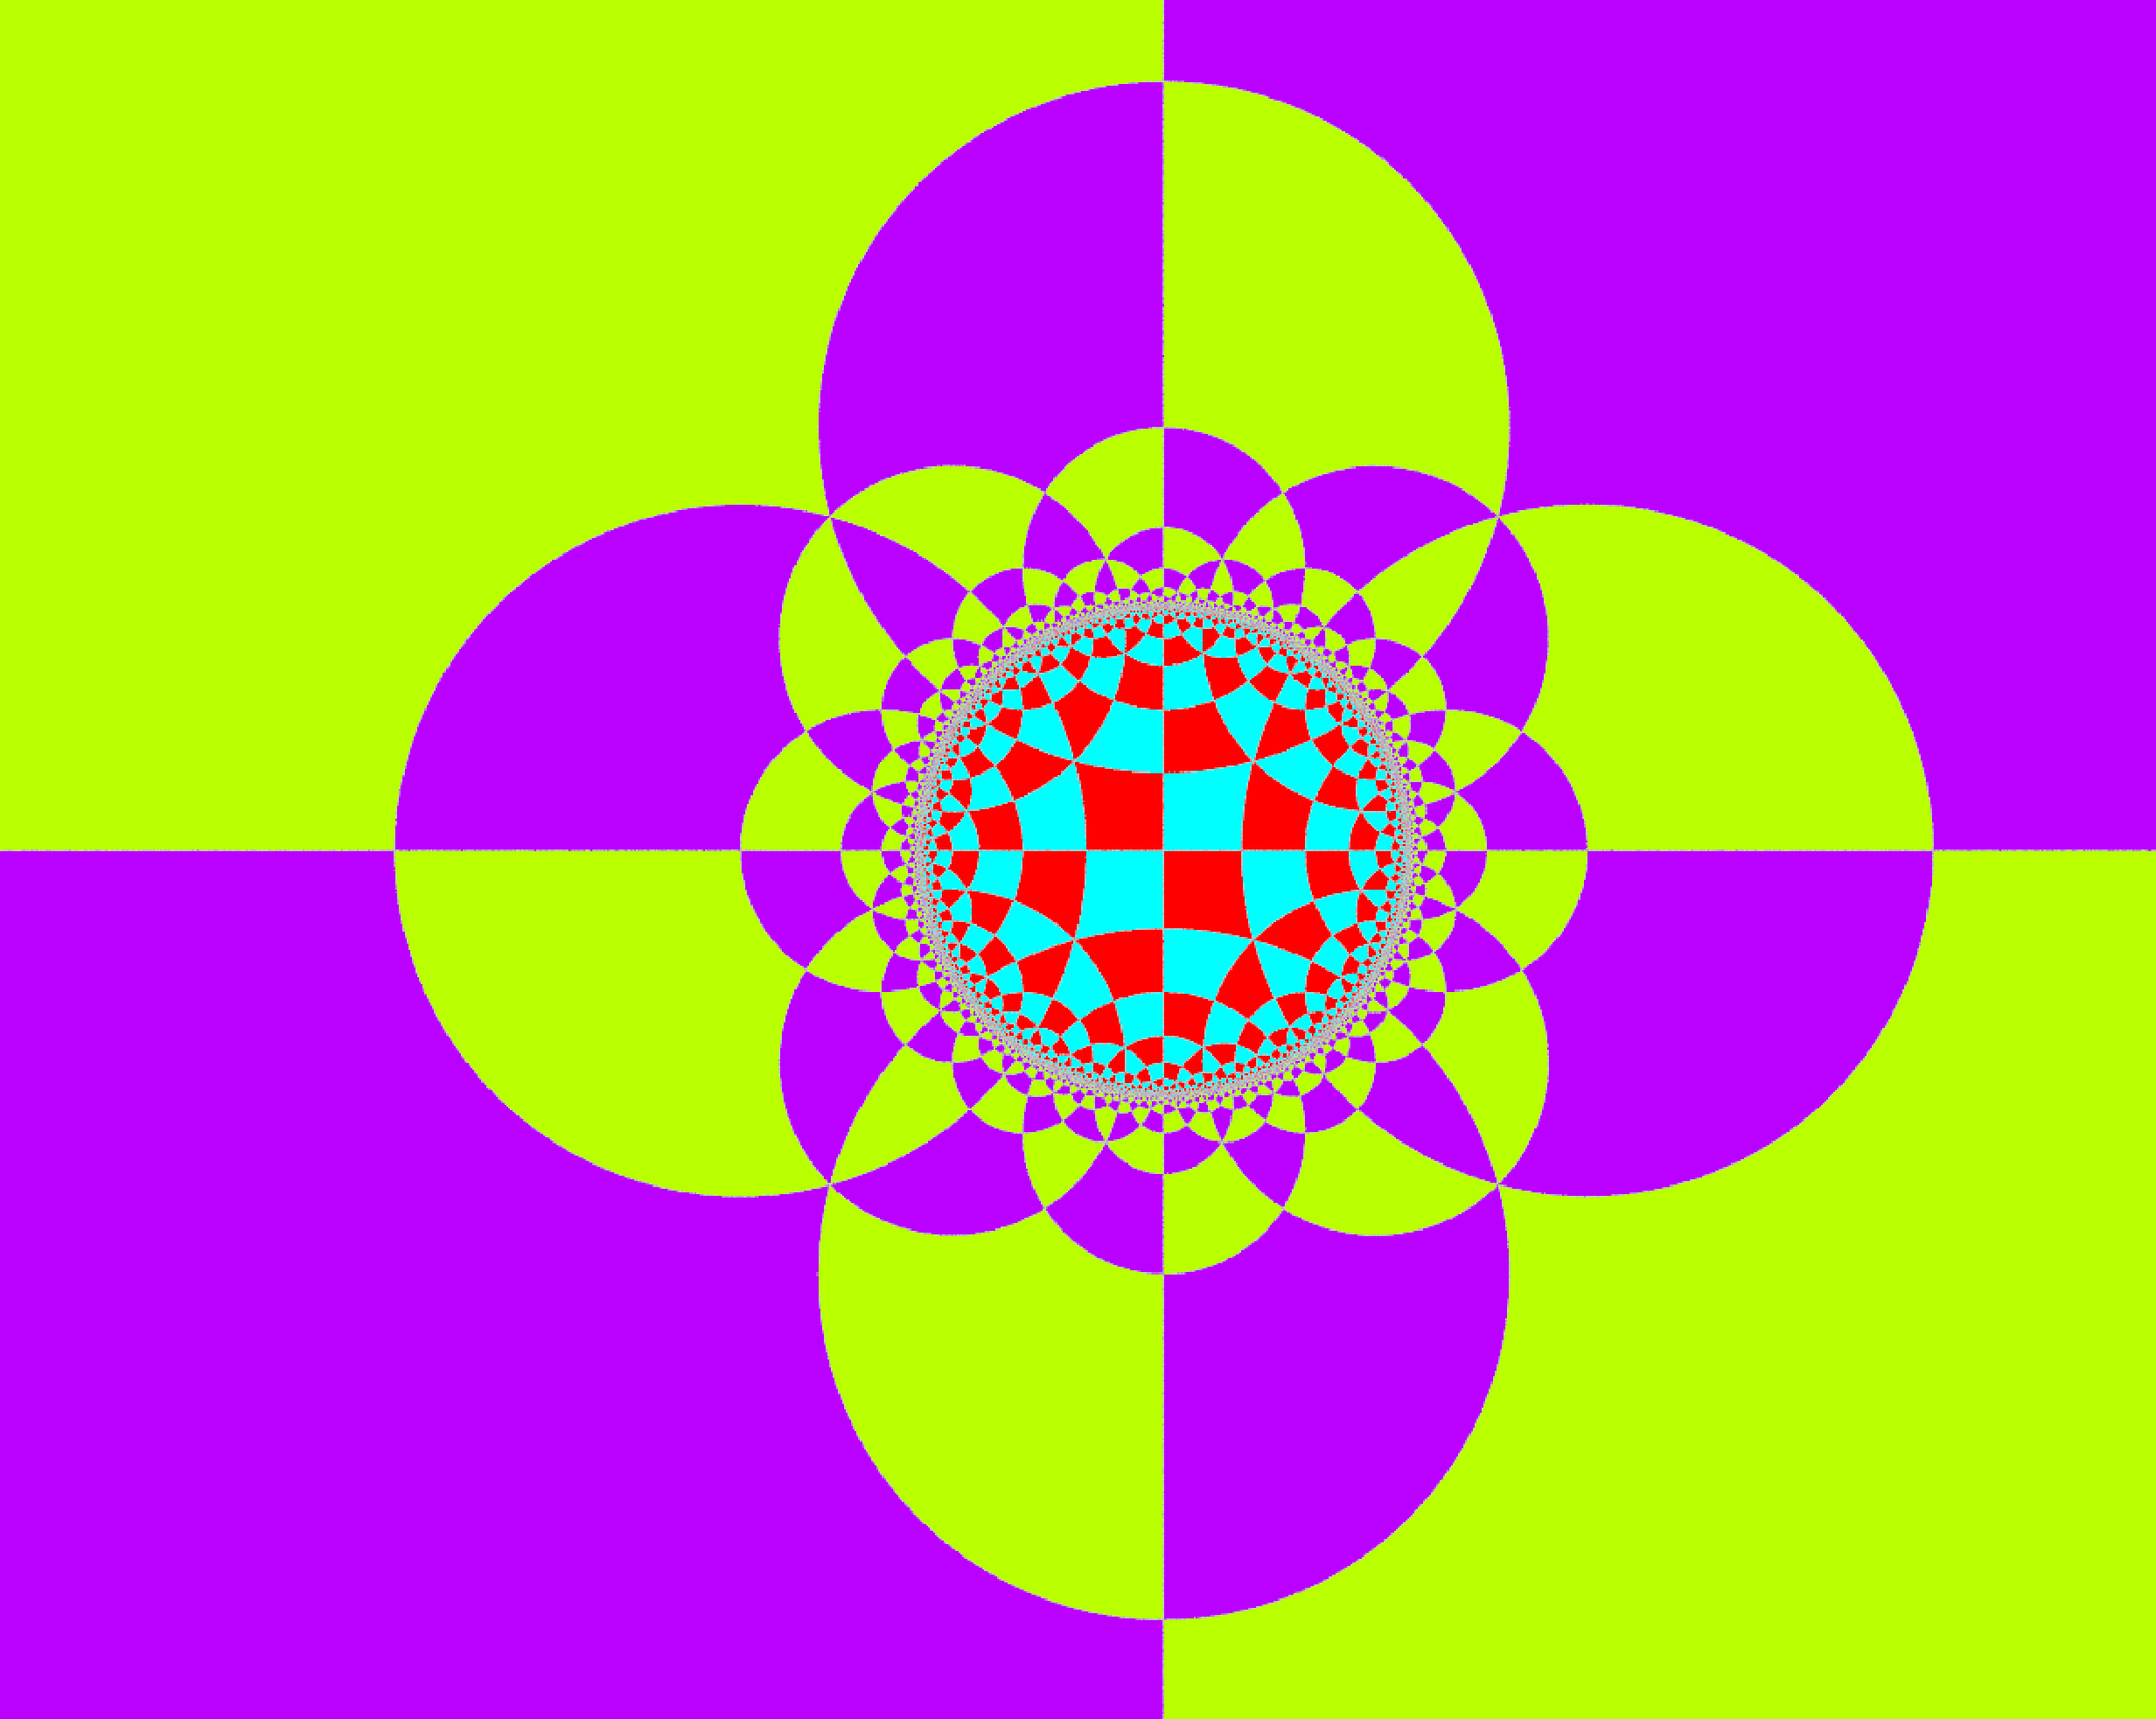
\includegraphics[width=3in, height=3in, keepaspectratio]{../img/tessellation/outer.pdf}
    \caption{Hyperbolic Tessellation}
    \label{fig:outer}
   \end{center}
 \end{minipage}
\end{figure}


\begin{figure}[htbp]
 \begin{center}
      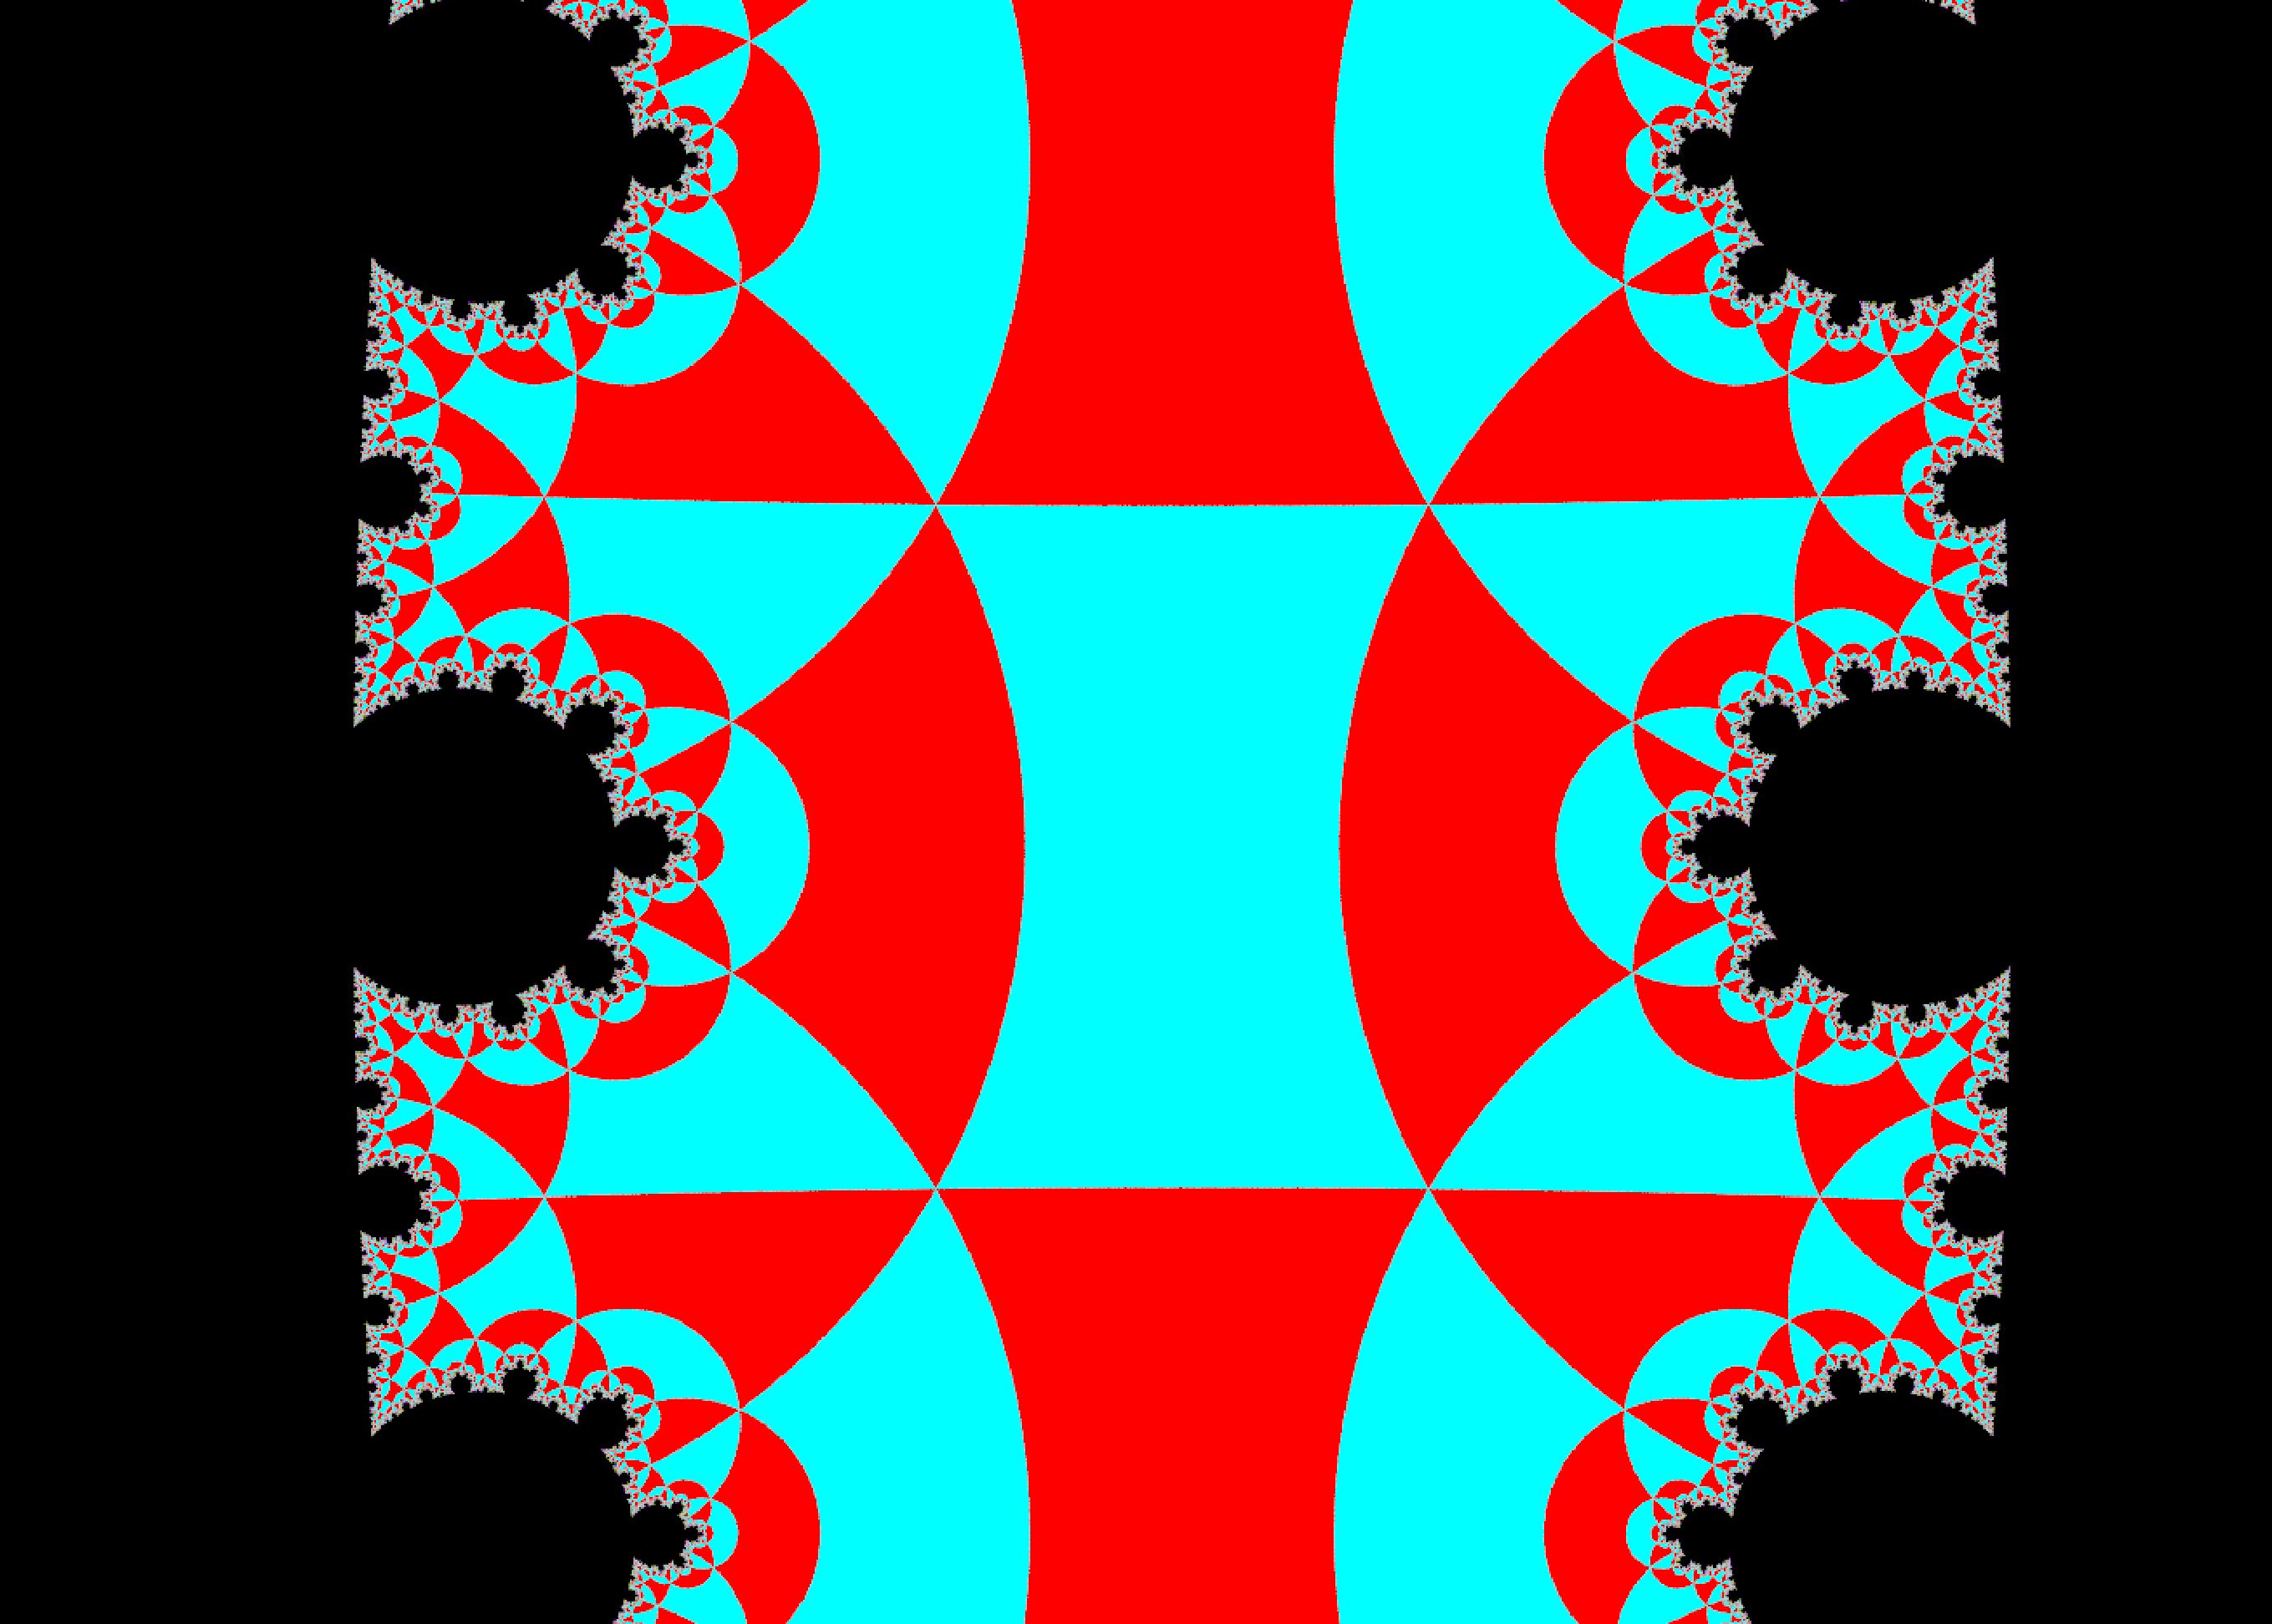
\includegraphics[width=3in, height=3in, keepaspectratio]{../img/tessellation/deformedTessellation.pdf}
    \caption{deformed}
    \label{fig:deformed}
 \end{center}
\end{figure}
